% Copyright 2012 David W. Hogg (NYU).  All rights reserved.

\documentclass[pdftex]{beamer}
\usepackage{amssymb,amsmath,mathrsfs}
\usecolortheme{default}

% this one is debatable
\renewcommand{\emph}[1]{\textbf{#1}}

%%% color commands
\newcommand{\whiteonblack}{%
  \colorlet{fg}{white}
  \colorlet{bg}{black}
  \setbeamercolor{normal_text}{fg=white,bg=black}
  \setbeamercolor{background canvas}{fg=white,bg=black}
  \setbeamercolor{alerted_text}{fg=yellow}
  \setbeamercolor{example_text}{fg=white}
  \setbeamercolor{structure}{fg=white}
  \setbeamercolor{palette_quaternary}{fg=white}
}
\newcommand{\blackonwhite}{%
  \colorlet{fg}{black}
  \colorlet{bg}{white}
  \setbeamercolor{normal_text}{fg=black,bg=white}
  \setbeamercolor{background canvas}{fg=black,bg=white}
  \setbeamercolor{alerted_text}{fg=blue}
  \setbeamercolor{example_text}{fg=black}
  \setbeamercolor{structure}{fg=black}
  \setbeamercolor{palette_quaternary}{fg=black}
}
\xdefinecolor{pink}{rgb}{1.0,0.9,0.9}

%%% size and shape commands
\newlength{\figurewidth}
\setlength{\figurewidth}{0.9\textwidth}
\newlength{\figureheight}
\setlength{\figureheight}{0.9\textheight}

%%% text commands
\newcommand{\project}[1]{\textsl{#1}}
  \newcommand{\an}{\project{Astrometry.net}}
  \newcommand{\tc}{\project{The~Cannon}}
  \newcommand{\euclid}{\project{Euclid}}
  \newcommand{\flickr}{\project{flickr}}
  \newcommand{\gaia}{\project{Gaia}}
  \newcommand{\galex}{\project{GALEX}}
  \newcommand{\kepler}{\project{Kepler}}
  \newcommand{\GALEX}{\galex}
  \newcommand{\hst}{\project{HST}}
  \newcommand{\hipparcos}{\project{Hipparcos}}
  \newcommand{\lsst}{\project{LSST}}
  \newcommand{\sdss}{\project{SDSS}}
  \newcommand{\sdssiii}{\project{SDSS-III}}
  \newcommand{\sdssiv}{\project{SDSS-IV}}
  \newcommand{\boss}{\sdssiii\ \project{BOSS}}
  \newcommand{\osss}{\project{OSSS}}
  \newcommand{\ska}{\project{SKA}}
  \newcommand{\vo}{\project{VO}}
  \newcommand{\rttd}{\project{Right Thing To Do}$^{\mbox{\scriptsize\sffamily{TM}}}$}
\newcommand{\foreign}[1]{\textit{#1}}
\newcommand{\latin}[1]{\foreign{#1}}
  \newcommand{\cf}{\latin{cf.}}
  \newcommand{\eg}{\latin{e.g.}}
  \newcommand{\etal}{\latin{et~al.}}
  \newcommand{\etc}{\latin{etc.}}
  \newcommand{\ie}{\latin{i.e.}}
  \newcommand{\vs}{\latin{vs.}}

%%% math-mode commands
\newcommand{\unit}[1]{\mathrm{#1}}
  \newcommand{\rad}{\unit{rad}}
  \newcommand{\s}{\unit{s}}
  \newcommand{\yr}{\unit{yr}}
  \newcommand{\km}{\unit{km}}
  \newcommand{\kmps}{\km\,\s^{-1}}
\newcommand{\mmatrix}[1]{\boldsymbol{#1}}
\newcommand{\tv}[1]{\boldsymbol{#1}}
\newcommand{\dd}{\mathrm{d}}
\newcommand{\given}{\,|\,}
\newcommand{\Teff}{T_{\mathrm{eff}}}
\newcommand{\logg}{\log g}
\newcommand{\vsini}{v\,\sin i}
 % hogg standard colors
\usepackage{amssymb,amsmath,mathrsfs}

\title{Going beyond map--reduce and going beyond maximum-likelihood}
\author[David W. Hogg (NYU)]{David W. Hogg \\
  \textsl{\small Center for Cosmology and Particle Physics,
                 New York University}}
\date{2012 September 11}

\newcommand{\conclusion}{
\blackonwhite
\setbeamercolor{background canvas}{bg=pink}
\begin{frame}
  \frametitle{Punchlines}
  \begin{itemize}
  \item The map--reduce framework (or something like it) does
    complicated tasks in $\log N$ time; it is the ``only'' framework
    for big data operations at the present day.
  \item The next generation of astronomy projects have to go beyond
    maximum-likelihood methods to more responsible probabilistic
    methods if they are going to deliver on their promises.
    \begin{itemize}
    \item \gaia, \lsst, \euclid, \etc
    \end{itemize}
  \item We don't know how to do much beyond maximum likelihood
    ``at scale''.
    \begin{itemize}
    \item call to arms
    \item (and get rich too!)
    \end{itemize}
  \end{itemize}
\end{frame}
\blackonwhite
}

\begin{document}

\blackonwhite

\begin{frame}
  \titlepage
\end{frame}

\conclusion

\begin{frame}
  \frametitle{Principal collaborators}
  \begin{itemize}
  \item Rob Fergus (NYU)
  \item Dan Foreman-Mackey (NYU)
  \item Dustin Lang (CMU)
  \end{itemize}
\end{frame}

\begin{frame}
  \frametitle{map--reduce or die}
  \begin{itemize}
  \item \emph{``We can't run any algorithms that can't be written in the map-reduce framework.''}
  \item map:
    \begin{itemize}
    \item at each ``data point'' (on the distributed system), do an operation on that datum, produce output
    \item think: Search document for ``kittens'' and return DocumentID and PageRank if it hits.
    \end{itemize}
  \item reduce:
    \begin{itemize}
    \item between each pair of outputs, do an operation and return one new output, recurse up the tree
    \item think: compare two PageRanks and return DocumentID and PageRank of the better.
    \end{itemize}
  \item Brilliant.  And a huge opportunity.
  \end{itemize}
\end{frame}

\begin{frame}
  \frametitle{maximum-likelihood and map--reduce}
  \begin{itemize}
  \item full-data likelihood: $\displaystyle p(D\given\theta) =
    \prod_n p(d_n\given\theta)$
  \item Find the \emph{maximum with respect to $\theta$} of this
    likelihood.
  \item map:
    \begin{itemize}
    \item compute $\displaystyle\frac{\dd \ln p(d_n\given\theta)}{\dd\theta}$
    \end{itemize}
  \item reduce:
    \begin{itemize}
    \item pairwise sum
    \end{itemize}
  \item Go uphill.  Repeat as necessary; each iteration only takes
    $\log N$ time.
  \end{itemize}
\end{frame}

\begin{frame}
  \frametitle{astronomical scale}
  \begin{itemize}
  \item \lsst: $10^{10}$ galaxies in $10^{14}$ pixels
    \begin{itemize}
    \item get the cosmic shear map
    \item and then the cosmological parameters
    \end{itemize}
  \item \gaia: $10^{9}$ stars in $10^{12}$ pixels
    \begin{itemize}
    \item infer the dynamics of the Milky Way
    \item but also---necessarily---the distribution function of stars
      in that potential
    \end{itemize}
  \item \emph{non-parametric} shear map or distribution function
    \begin{itemize}
    \item ``non-parametric'' means the model \emph{gets bigger as the
      data set gets bigger}
    \item importantly, non-parametric models are \emph{never} inferred
      at high signal-to-noise
    \end{itemize}
  \end{itemize}
\end{frame}

\begin{frame}
  \frametitle{graphical models}
\end{frame}

\begin{frame}
  \frametitle{astrophysics problems are hierarchical}
\end{frame}

\begin{frame}
  \frametitle{there are no linear problems}
\end{frame}

\begin{frame}
  \frametitle{marginalization is a bitch---and unavoidable}
\end{frame}

\begin{frame}
  \frametitle{Bayesian inference \emph{looks} map--reduce}
\end{frame}

\conclusion

\end{document}

\begin{frame}
  \frametitle{}
\end{frame}

\begin{frame}
  \frametitle{What is inference?}
  \begin{itemize}
  \item I have some data $\tv{D}$, I need to measure $x$.
  \item theoretically inspired arithmetic operations on the data?
  \item maximum-likelihood estimator?
  \item \emph{No: full likelihood function} $p(\tv{D}|x,\tv{\alpha})$
  \item \emph{And} marginalize $p(\tv{D}|x) = \int p(\tv{D}|x,\tv{\alpha})\,p(\tv{\alpha})\,\dd\tv{\alpha}$
    \begin{itemize}
    \item like a rotation and projection of the data into the $x$ space
    \item as lossless as possible (there are theorems)
    \item likelihoods can be combined with other likelihoods to
      correctly combine multiple data sets relevant to $x$.
    \end{itemize}
  \end{itemize}
\end{frame}

\begin{frame}
  \frametitle{1. Data-driven models}
\end{frame}

\end{document}

\begin{frame}
  \frametitle{extreme deconvolution {\small (Bovy, Hogg, Roweis 0905.2979)}: demo}
  \includegraphics[width=\textwidth]{toy-xd-sample.png}
\end{frame}
\begin{frame}
  \frametitle{extreme deconvolution {\small (Bovy, Hogg, Roweis 0905.2979)}: demo}
  \includegraphics[width=\textwidth]{toy-xd-hist.png}
\end{frame}
\begin{frame}
  \frametitle{extreme deconvolution {\small (Bovy, Hogg, Roweis 0905.2979)}: demo}
  \includegraphics[width=\textwidth]{toy-xd-01.png}
\end{frame}
\begin{frame}
  \frametitle{extreme deconvolution {\small (Bovy, Hogg, Roweis 0905.2979)}: demo}
  \includegraphics[width=\textwidth]{toy-xd-00.png}
\end{frame}
\begin{frame}
  \frametitle{extreme deconvolution {\small (Bovy, Hogg, Roweis 0905.2979)}: demo}
  \includegraphics[width=\textwidth]{toy-xd-02.png}
\end{frame}
\begin{frame}
  \frametitle{extreme deconvolution {\small (Bovy, Hogg, Roweis 0905.2979)}: demo}
  \includegraphics[width=\textwidth]{toy-xd-03.png}
\end{frame}
\begin{frame}
  \frametitle{extreme deconvolution {\small (Bovy, Hogg, Roweis 0905.2979)}: demo}
  \includegraphics[width=\textwidth]{toy-xd-04.png}
\end{frame}
\begin{frame}
  \frametitle{extreme deconvolution {\small (Bovy, Hogg, Roweis 0905.2979)}: demo}
  \includegraphics[width=\textwidth]{toy-xd-05.png}
\end{frame}
\begin{frame}
  \frametitle{extreme deconvolution {\small (Bovy, Hogg, Roweis 0905.2979)}: demo}
  \includegraphics[width=\textwidth]{toy-xd-06.png}
\end{frame}
\begin{frame}
  \frametitle{extreme deconvolution {\small (Bovy, Hogg, Roweis 0905.2979)}: demo}
  \includegraphics[width=\textwidth]{toy-xd-07.png}
\end{frame}
\begin{frame}
  \frametitle{extreme deconvolution {\small (Bovy, Hogg, Roweis 0905.2979)}: demo}
  \includegraphics[width=\textwidth]{toy-xd-08.png}
\end{frame}
\begin{frame}
  \frametitle{extreme deconvolution {\small (Bovy, Hogg, Roweis 0905.2979)}: demo}
  \includegraphics[width=\textwidth]{toy-xd-09.png}
\end{frame}
\begin{frame}
  \frametitle{extreme deconvolution {\small (Bovy, Hogg, Roweis 0905.2979)}: demo}
  \includegraphics[width=\textwidth]{toy-xd-sample.png}
\end{frame}
\begin{frame}
  \frametitle{extreme deconvolution {\small (Bovy, Hogg, Roweis 0905.2979)}: idea}
  \begin{itemize}
  \item Each datum $x_n$ has its own error $\sigma_n$, therefore
  \item each datum $x_n$ is drawn from it's own, individual pdf $p(x_n\given\sigma_n,\theta)$.
  \item Parameterize the true (zero-error) PDF with ``hyperparameters'' $\theta$ and
  \item find the hyperparameters that optimize the combined likelihood of \emph{all the data}.
      \begin{eqnarray}\displaystyle
      p(\left\{x_n\right\}\given\theta) &=& \prod_n p(x_n\given\sigma_n,\theta)
      \end{eqnarray}
  \item Generalize to $D$ dimensions.
  \end{itemize}
\end{frame}

\begin{frame}
  \frametitle{XDQSO {\small (Bovy \etal\ 1011.6392)}: setup}
  \begin{itemize}
  \item $2.2<z<3.5$ quasars can be used to measure the baryon acoustic
    oscillation in the Lyman alpha forest
  \item \project{SDSS-III BOSS}
  \item quasars in this range \emph{look like stars} in $ugriz$
  \item This is a hard supervised classification problem.
  \end{itemize}
\end{frame}

\begin{frame}
  \frametitle{XDQSO {\small (Bovy \etal\ 1011.6392)}: results}
\includegraphics[width=0.32\textwidth,clip=]{single_data_200_i_202_gr_ug.png}
\includegraphics[width=0.32\textwidth,clip=]{dc_fluxdist_resample_200_i_202_20_gr_ug.png}
\includegraphics[width=0.32\textwidth,clip=]{coadd_data_200_i_202_gr_ug.png}\\
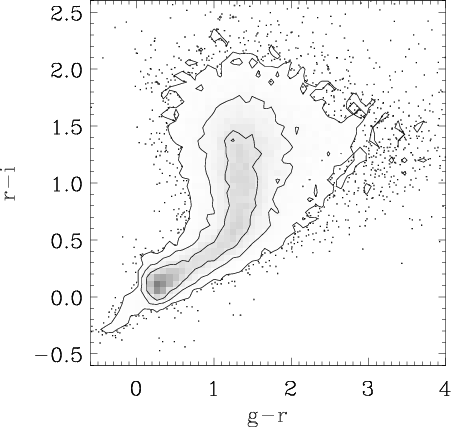
\includegraphics[width=0.32\textwidth,clip=]{single_data_200_i_202_ri_gr.png}
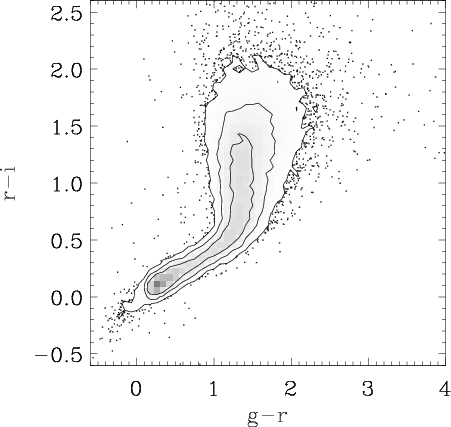
\includegraphics[width=0.32\textwidth,clip=]{dc_fluxdist_resample_200_i_202_20_ri_gr.png}
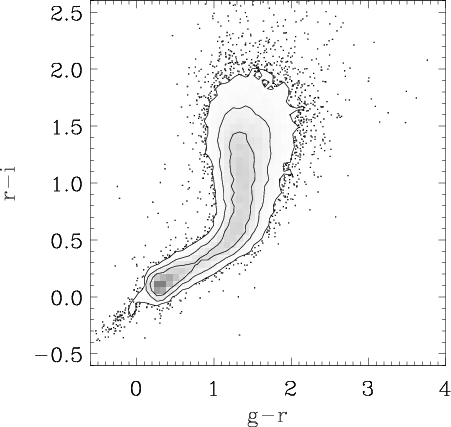
\includegraphics[width=0.32\textwidth,clip=]{coadd_data_200_i_202_ri_gr.png}\\
\includegraphics[width=0.32\textwidth,clip=]{single_data_200_i_202_iz_ri.png}
\includegraphics[width=0.32\textwidth,clip=]{dc_fluxdist_resample_200_i_202_20_iz_ri.png}
\includegraphics[width=0.32\textwidth,clip=]{coadd_data_200_i_202_iz_ri.png}
\end{frame}

\begin{frame}
  \frametitle{XDQSO {\small (Bovy \etal\ 1011.6392)}: results}
  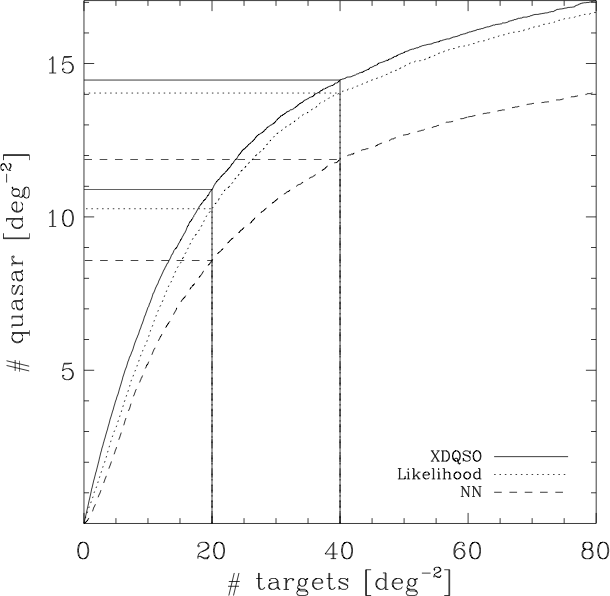
\includegraphics[height=\figureheight]{xdqso_performance.png}
\end{frame}

\begin{frame}
  \frametitle{XDQSO {\small (Bovy \etal\ 1011.6392)}: why do we win?}
  \begin{itemize}
  \item We are data-driven.
  \item We use the errors correctly and account properly for missing
    data; we have a \emph{generative model}.
  \item That is true for both the training data and the test data.
  \item We are extensible to new prior information or other data.
    \begin{itemize}
    \item \project{GALEX}
    \item \project{UKIDSS}
    \item variability
    \end{itemize}
  \item \project{extreme-deconvolution}
    \begin{itemize}
    \item Bovy, Hogg, \& Roweis (0905.2979)
    \item it Just Works (tm)
    \item C code with Python and IDL wrappers / interface
    \item can handle large data sets with large numbers of dimensions
    \end{itemize}
  \item \project{SDSS-III} \project{BOSS} core target selection
  \end{itemize}
\end{frame}

\begin{frame}
  \frametitle{Polemic: What's wrong with typical classification algorithms?}
  \begin{itemize}
  \item neural networks, boltzmann machines, support vector machines, boosting
  \item these are all \emph{awesome}
  \item they require that \emph{test data} have the same statistical
    and error properties as \emph{training data} \\
    \emph{never true!}
  \item they require that all features be measured for all data points \\
    \emph{never true!}
  \end{itemize}
\end{frame}

\begin{frame}
  \frametitle{XDQSOz redshift prediction {\small (Bovy \etal\ 1105.3975)}: example}
\includegraphics[height=0.9\textheight]{./predict_dr7qso_sdss.png}
\end{frame}

\begin{frame}
  \frametitle{XDQSOz redshift prediction {\small (Bovy \etal\ 1105.3975)}: example}
  \includegraphics[height=0.9\textheight]{./predict_dr7qso_galex.png}
\end{frame}

\begin{frame}
  \frametitle{XDQSOz redshift prediction {\small (Bovy \etal\ 1105.3975)}: example}
  \includegraphics[height=0.9\textheight]{./predict_dr7qso_ukidss.png}
\end{frame}

\begin{frame}
  \frametitle{XDQSOz redshift prediction {\small (Bovy \etal\ 1105.3975)}: example}
  \includegraphics[height=0.9\textheight]{./predict_dr7qso_galex_ukidss.png}
\end{frame}

\begin{frame}
  \frametitle{XDQSOz redshift prediction {\small (Bovy \etal\ 1105.3975)}: lessons}
  \begin{itemize}
  \item When you have a probabilistic generative model, generating the
    raw data, even \emph{extremely low signal-to-noise data can be
      decisive}.
  \item Catalogs are useless in this regime.
  \end{itemize}
\end{frame}

\begin{frame}
  \frametitle{High contrast imaging {\small (Fergus \etal)}: examples}
  \includegraphics[width=\textwidth]{fergus-examples.pdf}\\
  data from the \project{P1640} spectroscopic imaging coronograph {\small (Oppenheimer \etal)}
  \begin{itemize}
  \item Data are four dimensional: $x$, $y$, $\lambda$, $n_{\mathrm exp}$.
  \item Expect strong structure in the radius--wavelength plane.
  \end{itemize}
\end{frame}
\begin{frame}
  \frametitle{High contrast imaging {\small (Fergus \etal)}: eigenvectors}
  \includegraphics[height=0.9\textheight]{fergus-eigenvectors.pdf}
\end{frame}
\begin{frame}
  \frametitle{High contrast imaging {\small (Fergus \etal)}: sensitivity}
  \includegraphics[width=0.92\textwidth]{fergus-maps.pdf}
\end{frame}

\begin{frame}
  \frametitle{Binary quasars {\small (Tsalmantza \etal\ 1106.1180)}: example}
  \includegraphics[width=\textwidth]{superposition_QG.pdf}
\end{frame}

\conclusion

\begin{frame}
  \frametitle{2. Foreground-background modeling}
\end{frame}

\begin{frame}
  \frametitle{GD-1 stream {\small (Grillmair \& Dionatos 2006 \textit{ApJL} \textbf{643} L17--L20.)}}
  \resizebox{\textwidth}{!}{\includegraphics{../gaia/grillmair.jpg}}
\end{frame}

\begin{frame}
  \frametitle{GD-1 stream {\small (Koposov \etal\ 0907.1085)}: setup}
  \resizebox{\textwidth}{!}{\includegraphics{koposov01.png}}
\end{frame}

\begin{frame}
  \frametitle{GD-1 stream {\small (Koposov \etal\ 0907.1085)}: results}
  \resizebox{!}{0.9\textheight}{\includegraphics{koposov06.png}}
\end{frame}

\begin{frame}
  \frametitle{GD-1 stream {\small (Koposov \etal\ 0907.1085)}: results}
  \resizebox{!}{0.9\textheight}{\includegraphics{koposov07.png}}
\end{frame}

\begin{frame}
  \frametitle{GD-1 stream {\small (Koposov \etal\ 0907.1085)}: lessons}
  \begin{itemize}
  \item We got the first-ever six-dimensional map of an orbit in the
    Milky Way.
  \item If we had required hard classification of every star, we
    would have \emph{failed}.
  \end{itemize}
\end{frame}

\begin{frame}
  \frametitle{Self-calibration of imaging {\small (Holmes, Rix, Hogg)}}
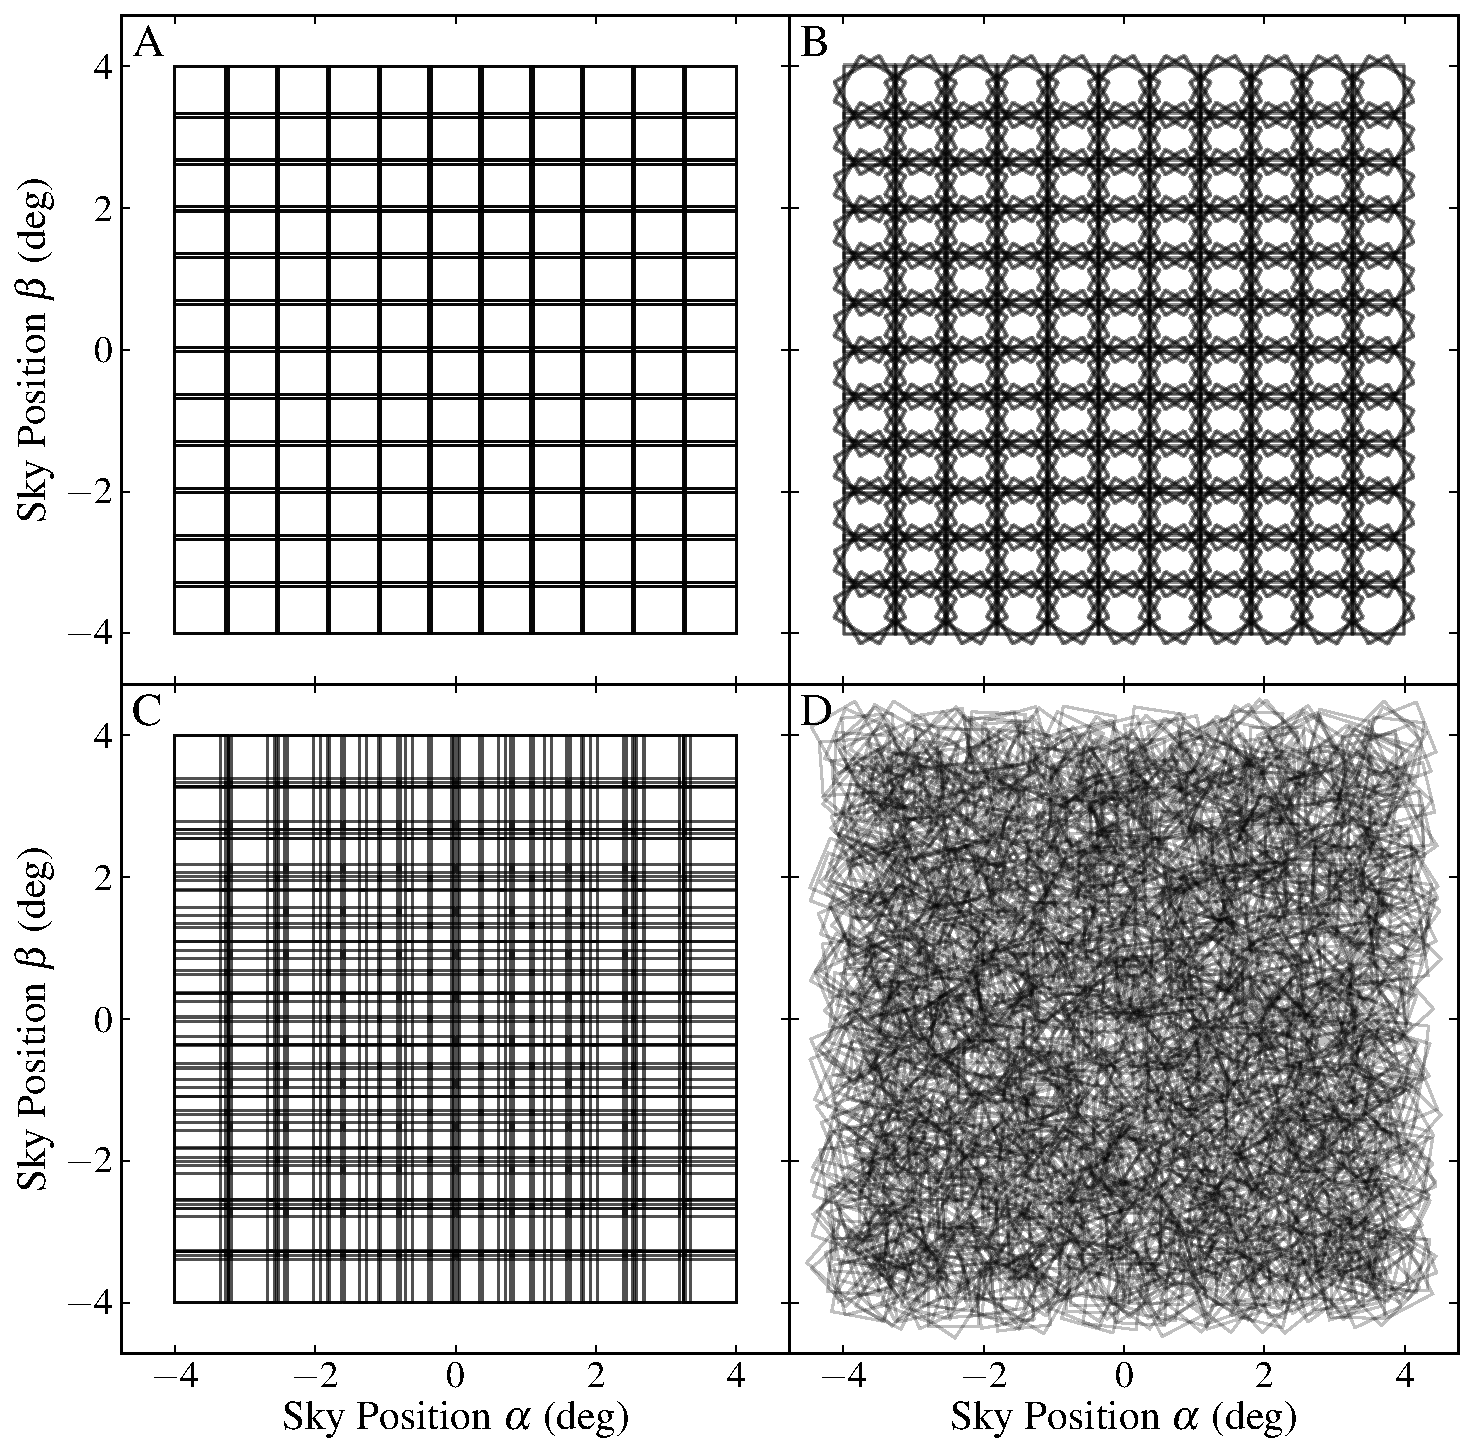
\includegraphics[height=0.9\textheight]{./simple_surveys.pdf}
\end{frame}

\begin{frame}
  \frametitle{Self-calibration of imaging {\small (Holmes, Rix, Hogg)}}
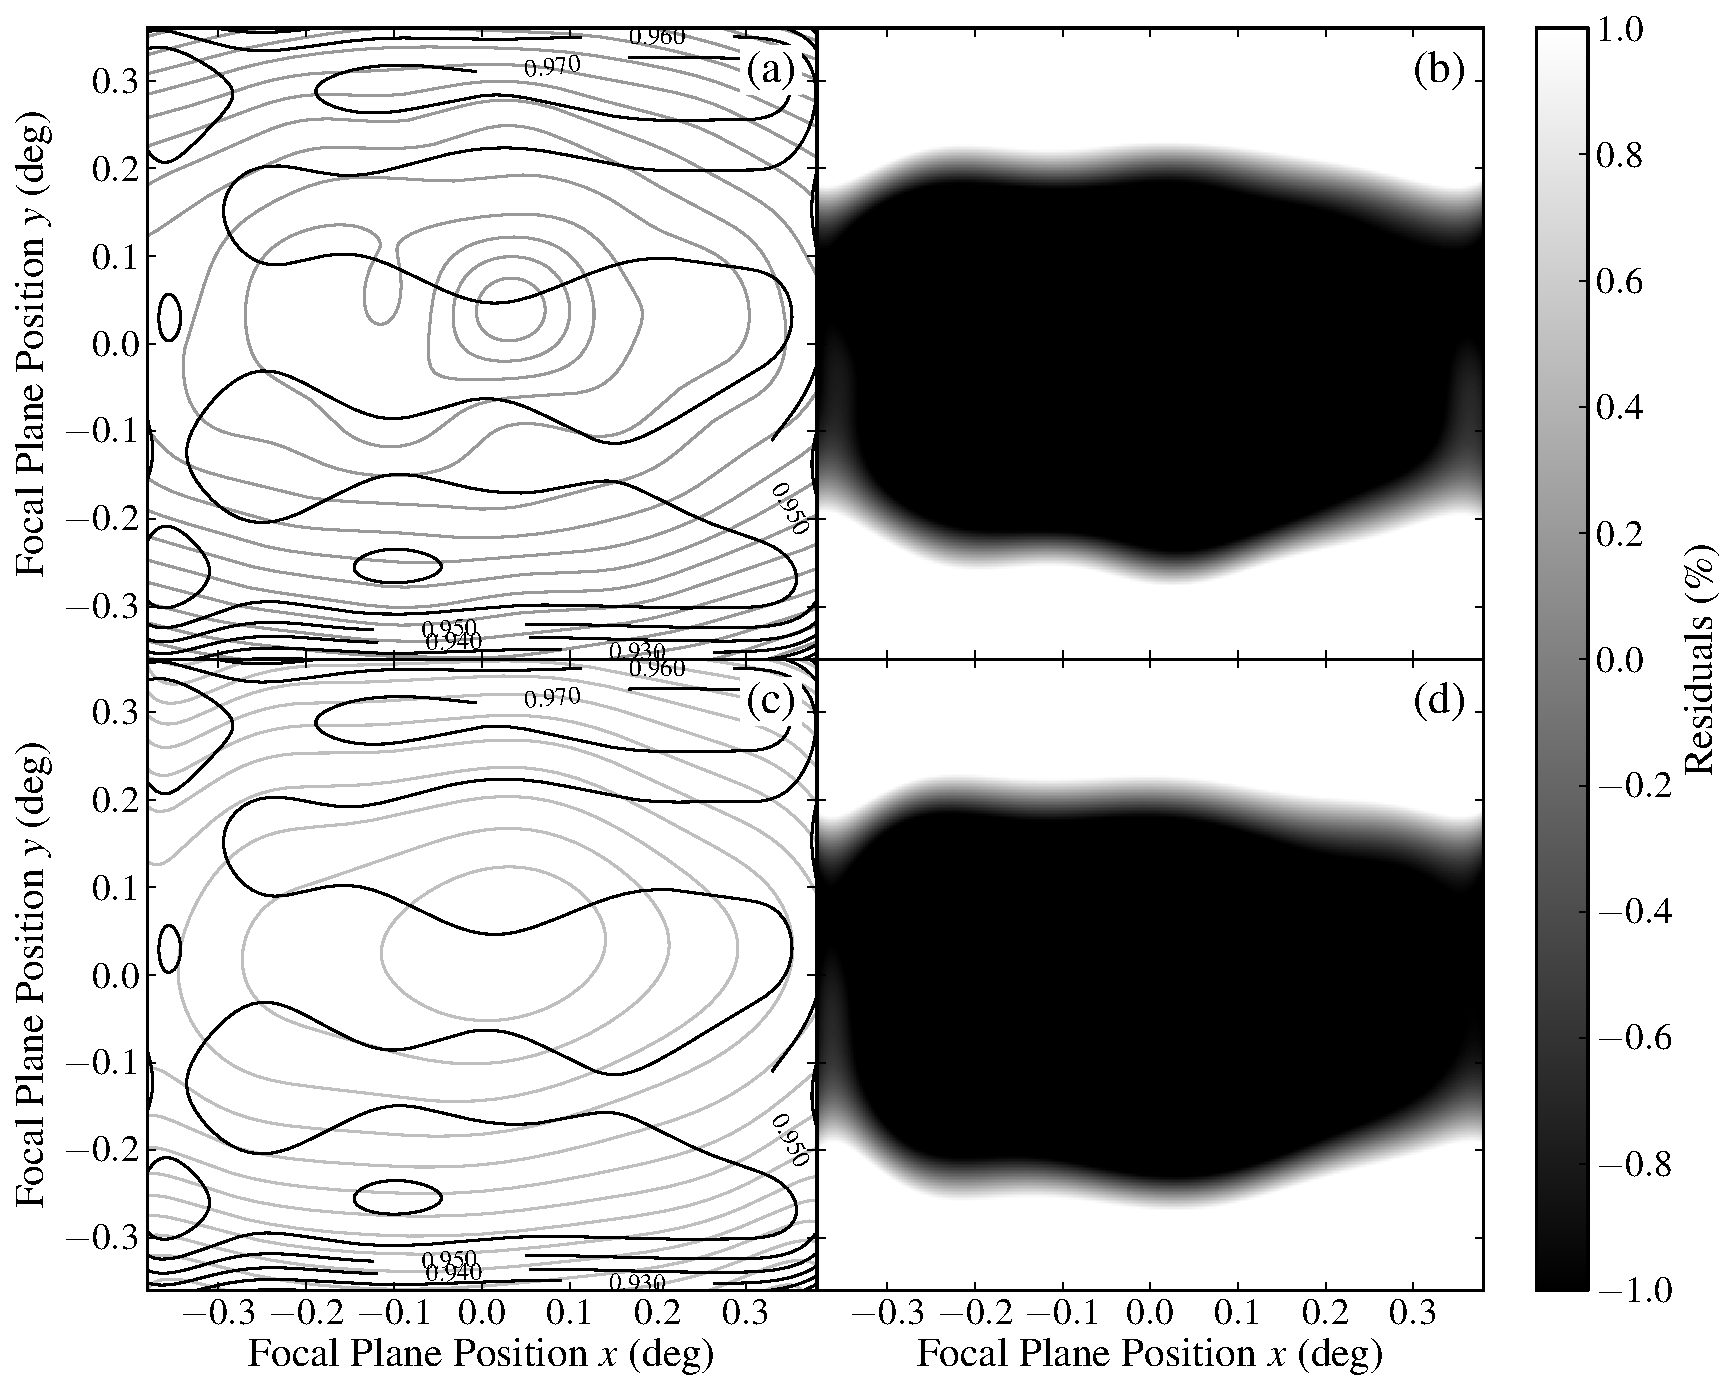
\includegraphics[height=0.44\textheight]{./A_8192_ff.pdf}
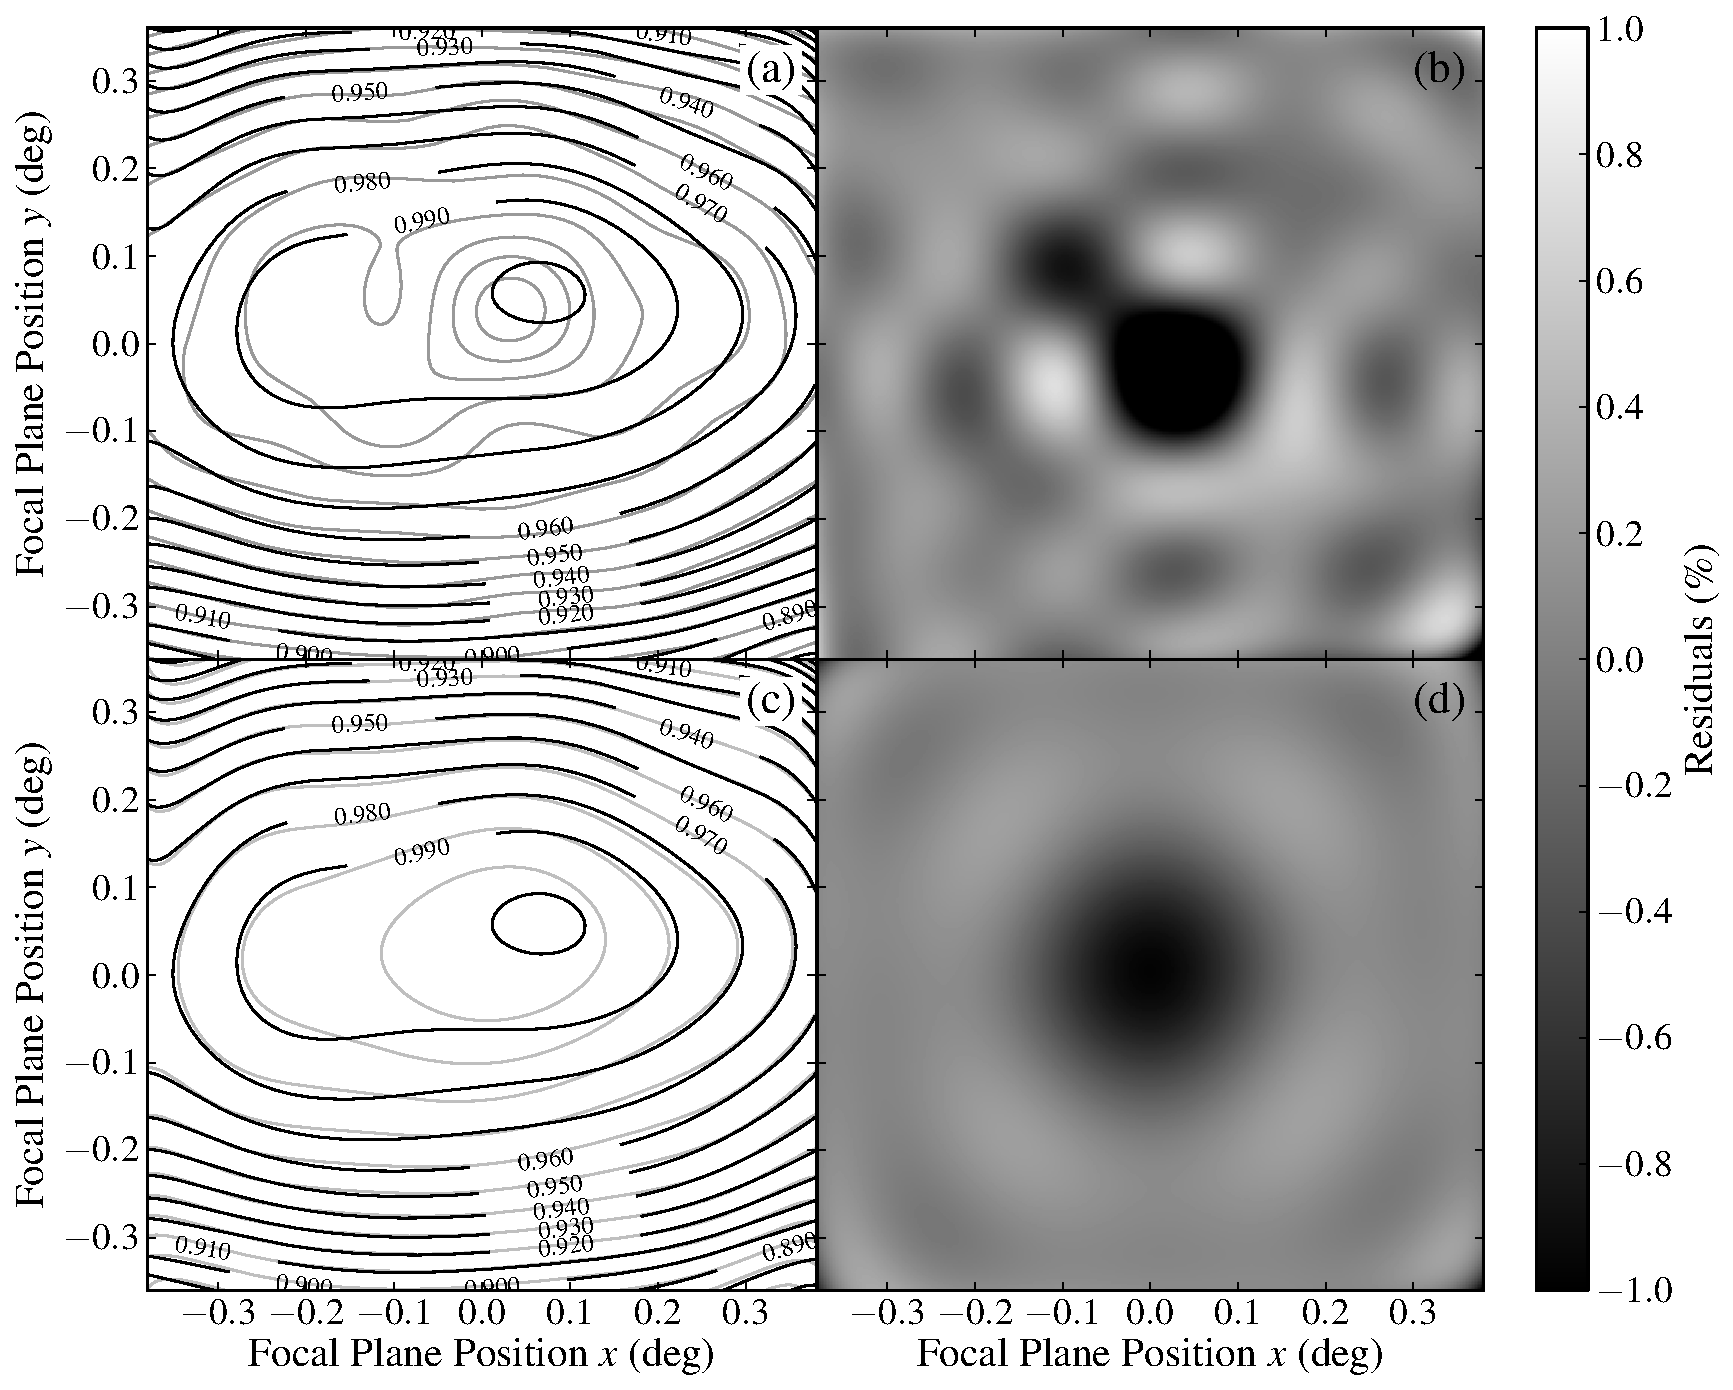
\includegraphics[height=0.44\textheight]{./B_4160_ff.pdf} \\
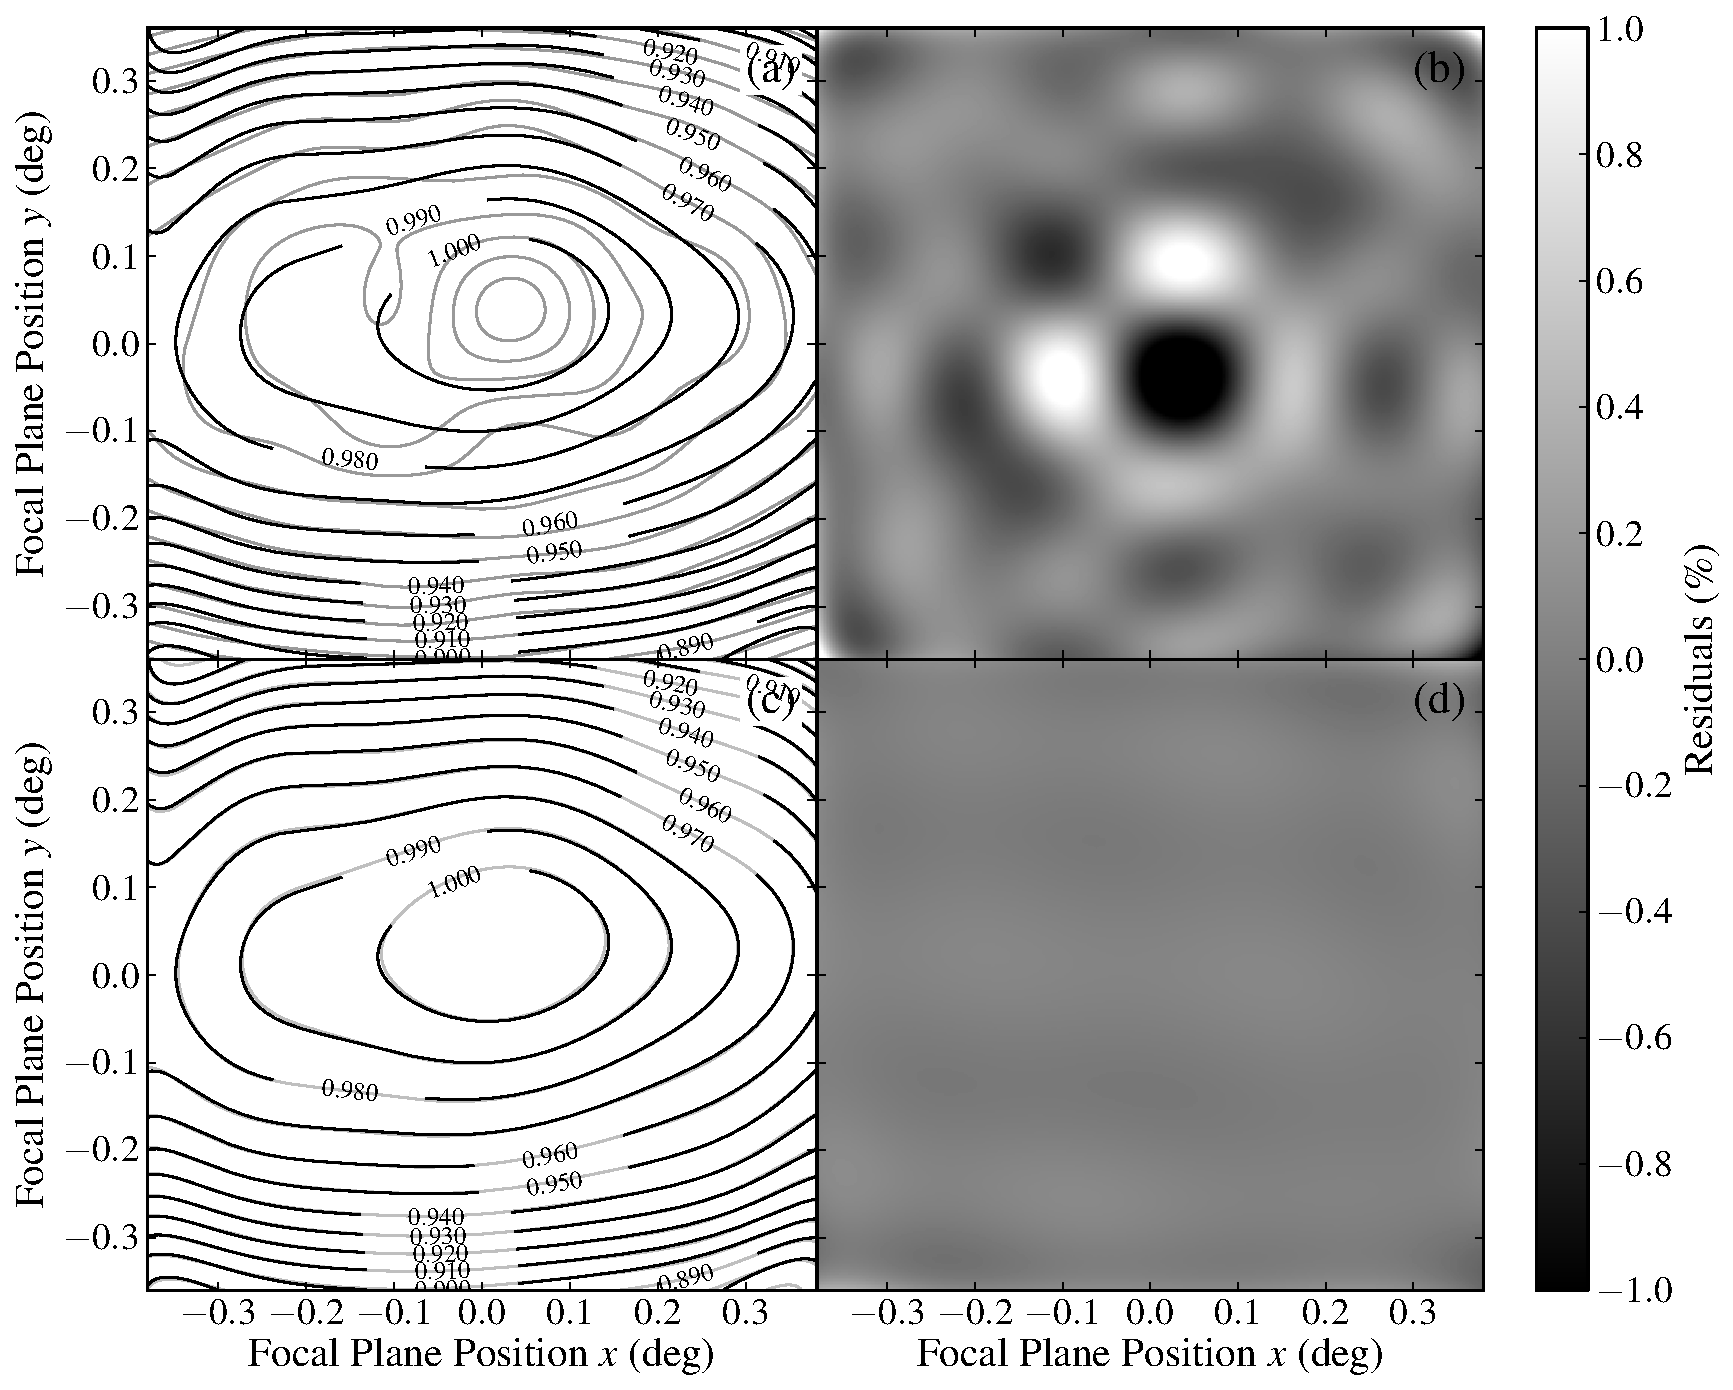
\includegraphics[height=0.44\textheight]{./C_026_ff.pdf}
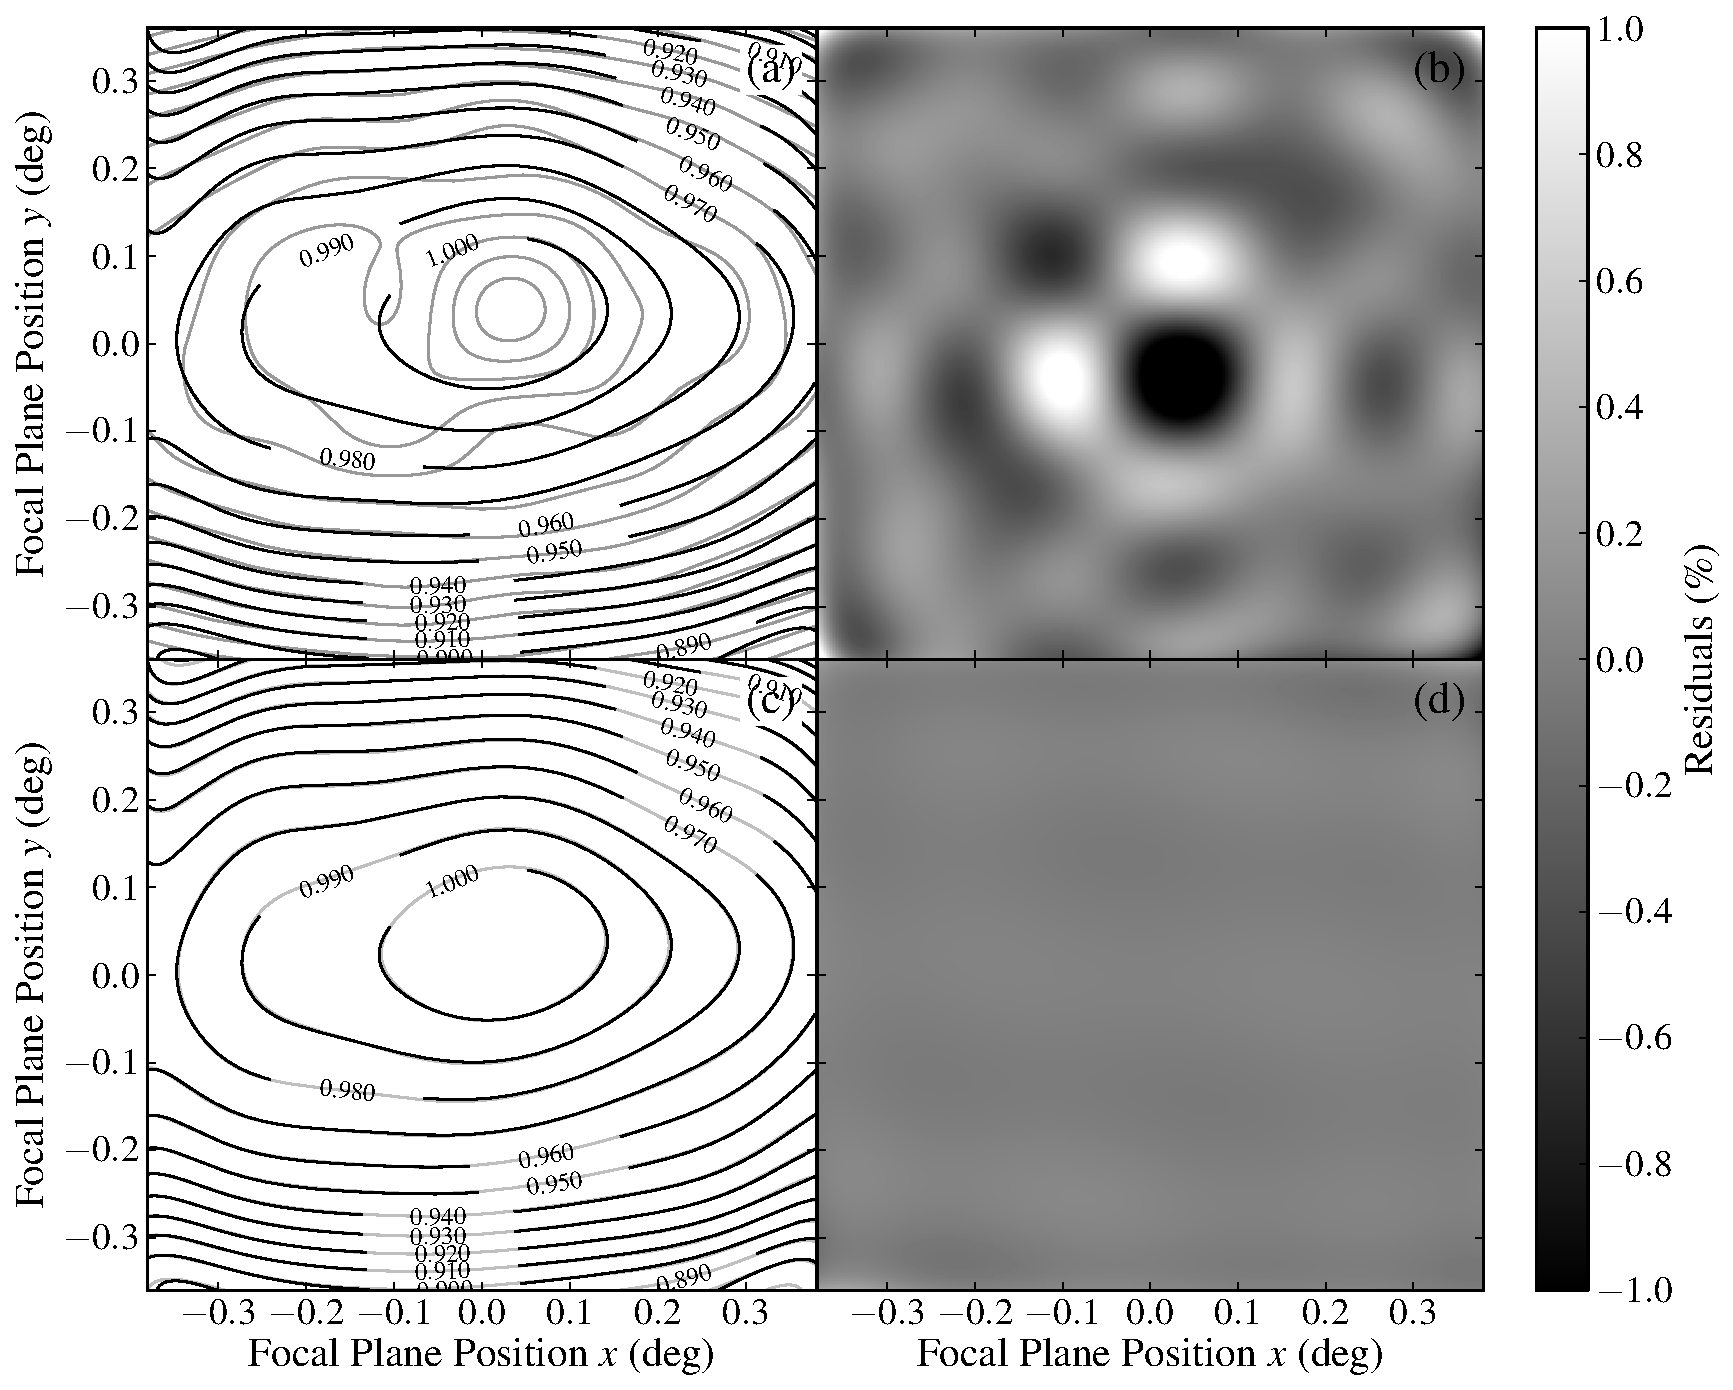
\includegraphics[height=0.44\textheight]{./D_009_ff.pdf}
\end{frame}

\begin{frame}
  \frametitle{Self-calibration of imaging}
  \begin{itemize}
  \item A good survey (Holmes \etal):
    \begin{itemize}
    \item every star appears in many images
    \item in different images, the star is in different places
    \item every image contains many stars
    \end{itemize}
  \item A good model (Foreman-Mackey \& Hogg):
    \begin{itemize}
    \item every star has some probability of being variable
    \item every datapoint has some probability of being corrupted
    \item calibrate without hard classification
    \item mixture model is a marginalization over good--bad decisions
    \item \emph{can recover many discarded SDSS-II Stripe 82 imaging runs}
    \end{itemize}
  \end{itemize}
\end{frame}

\conclusion

\begin{frame}
  \frametitle{3. Modeling the noise}
\end{frame}

\begin{frame}
  \frametitle{Exoplanets around white dwarfs {\small (Schiminovich, Lang, Hogg)}}
  \includegraphics[width=\textwidth]{model-1356.png}
\end{frame}
\begin{frame}
  \frametitle{Exoplanets around white dwarfs {\small (Schiminovich, Lang, Hogg)}}
  \includegraphics[height=0.9\textheight]{emcee_model_after.png}
\end{frame}
\begin{frame}
  \frametitle{Exoplanets around white dwarfs {\small (Schiminovich, Lang, Hogg)}}
  \includegraphics[width=\textwidth]{model-1380.png}
\end{frame}
\begin{frame}
  \frametitle{Exoplanets around white dwarfs {\small (Schiminovich, Lang, Hogg)}}
  \includegraphics[width=\textwidth]{model-1594.png}
\end{frame}
\begin{frame}
  \frametitle{Exoplanets around white dwarfs {\small (Schiminovich, Lang, Hogg)}}
  \includegraphics[width=\textwidth]{model-1659.png}
\end{frame}

\begin{frame}
  \frametitle{Exoplanets around red giants {\small (Hou, Goodman, Hogg)}}
  \includegraphics[width=\textwidth]{fits_1_planet_1_oscillation.png}
\end{frame}

\conclusion

\begin{frame}
  \frametitle{4. Catalogs are bad; unstacked images are good}
\end{frame}

\begin{frame}
  \frametitle{Faint proper motions {\small (Lang \etal\ 0808.4004)}: brown dwarf}
  \resizebox{0.60\textwidth}{!}{\includegraphics{faint-motion-1.png}} \\
\end{frame}

\begin{frame}
  \frametitle{Faint proper motions {\small (Lang \etal\ 0808.4004)}: $z>6$ QSO}
  \resizebox{0.60\textwidth}{!}{\includegraphics{faint-motion-2.png}}
\end{frame}

\begin{frame}
  \frametitle{Faint proper motions {\small (Lang \etal\ 0808.4004)}: faint galaxy}
  \resizebox{0.60\textwidth}{!}{\includegraphics{faint-motion-3.png}}
\end{frame}

\begin{frame}
  \frametitle{Faint proper motions {\small (Lang \etal\ 0808.4004)}: defect}
  \resizebox{0.60\textwidth}{!}{\includegraphics{faint-motion-4.png}}
\end{frame}

\begin{frame}
  \frametitle{Faint proper motions {\small (Lang \etal\ 0808.4004)}: lessons}
  \begin{itemize}
  \item If we had only a catalog, we would have \emph{failed}.
  \item If we had only a coadd, we would have \emph{failed}.
  \end{itemize}
\end{frame}

\begin{frame}
  \frametitle{What's wrong with \project{LSST} and \project{PanSTARRS}?}
  \begin{itemize}
  \item reducing data with point estimates
  \item building catalogs from ``co-adds'' with point estimates
  \item catalog matching
  \item \emph{All of these throw away information.  Does it matter?}
    \begin{itemize}
    \item Lang and I are betting it does: \project{theTractor.org}
    \end{itemize}
  \end{itemize}
\end{frame}

\begin{frame}
  \frametitle{The \project{Tractor} {\small (Lang \etal)}: data}
  \resizebox{1.1\textwidth}{!}{\includegraphics{s82-4858-1r-0348-data.png}}
\end{frame}

\begin{frame}
  \frametitle{The \project{Tractor} {\small (Lang \etal)}: model}
  \resizebox{1.1\textwidth}{!}{\includegraphics{s82-4858-1r-0348-model.png}}
\end{frame}

\conclusion

\begin{frame}
(backup slides)
\end{frame}

\begin{frame}
  \frametitle{The baryon acoustic feature}
  \begin{itemize}
    \item build galaxy catalog from noisy imaging and spectroscopy data
    \item build two-point function from catalog
    \item fit baryon acoustic feature to two-point function
    \item \emph{Can we write down the likelihood of the data instead?}
      \begin{itemize}
      \item model the density field
      \item model how galaxies populate that field
      \item enormous marginalization
      \item impossible? (\eg, Dodelson \etal\ 9712074)
      \end{itemize}
  \end{itemize}
\end{frame}

\begin{frame}
  \frametitle{Polemic: missing data}
  \begin{itemize}
  \item Most machine-learning methods hate missing data.
  \item Interpolation or data censoring (both very, very bad) are required.
  \item Any model that properly accounts for \emph{uncertainty} also
    properly accounts for \emph{missing data}.
    \begin{itemize}
    \item Missing data is (extreme) uncertainty; uncertainty is (mild)
      missing data.
    \end{itemize}
  \item If you have a justified generative model $p(\allvn|\allparsn)$,
    you automatically deal with missing data.
  \end{itemize}
\end{frame}

\begin{frame}
  \frametitle{Polemic: Don't convolve your data, convolve your model!}
  \begin{itemize}
  \item If you are uncertain about something (a redshift, a
    classification) so that you don't know which bin to put it in:
  \item \emph{Don't} put a bit of it into each bin!
    \begin{itemize}
    \item That re-convolves your noisy result with the noise again.
    \end{itemize}
  \item \emph{Do} put a bit of your \emph{distribution model} into each bin.
    \begin{itemize}
    \item That is, convolve your \emph{model} for the object with the uncertainty.
    \item Obvious, but frequently done wrong.
    \end{itemize}
  \end{itemize}
\end{frame}

\begin{frame}
  \frametitle{Polemic: Catalogs are dangerous {\small (Hogg \& Lang 1008.0738)}}
  \begin{itemize}
  \item No objects are detected or classified with perfect confidence.
  \item Different investigators have different objectives and priors.
  \item As new data become available, the balance will shift for many objects.
  \item \emph{Catalogs become wrong, likelihood \emph{functions} are forever.}
    \begin{itemize}
    \item and I mean \emph{functions}, not maxima
    \end{itemize}
  \end{itemize}
\end{frame}

\end{document}
